\clearpage
\section{The build}

\begin{figure}[H]
	\centering
	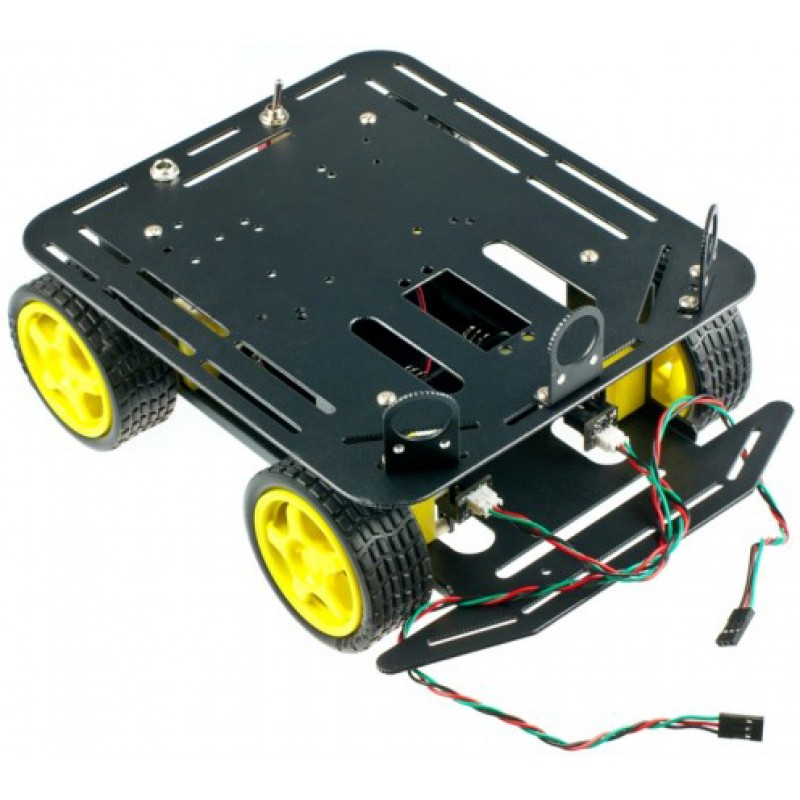
\includegraphics[width=.4\linewidth]{images/chassis.jpg}
\end{figure}

To attach the different sensors to the rover, different enclosures and brackets were needed. For the ultrasonic sensors, two different kind of brackets have been designed, since the main chassis required them to be mounted differently based on their placement on the chassis of the rover. Using Autodesk Inventor the two enclosures for the ultrasonic sensors have been modelled and 3D-printed.

\begin{figure}[H]
	\centering
	\begin{subfigure}[H]{0.4\textwidth}
		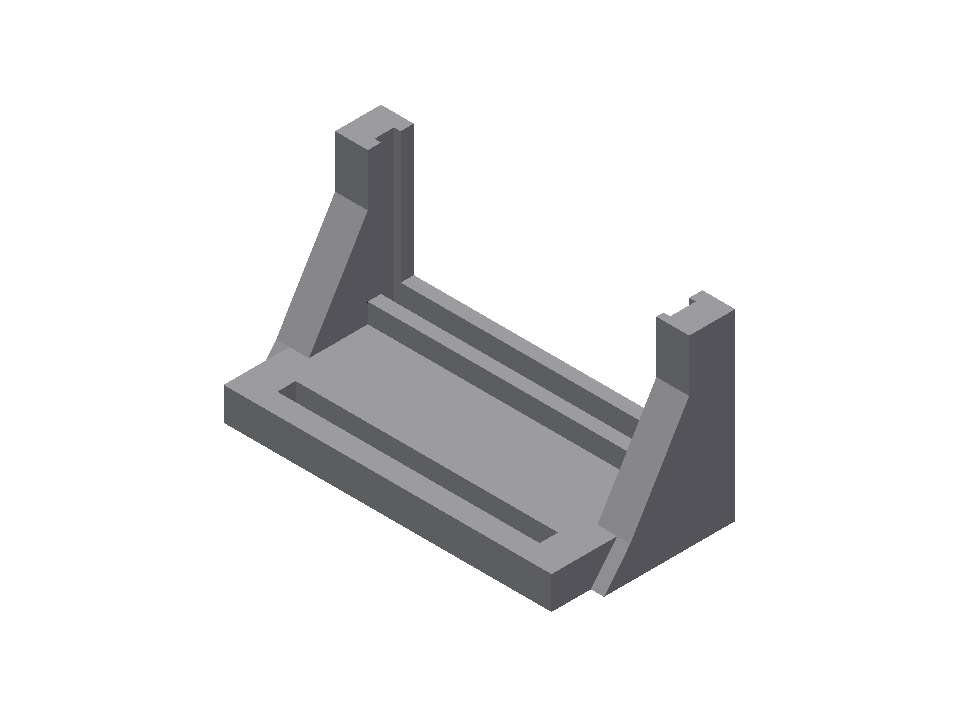
\includegraphics[width=\textwidth]{images/ultrasonicholder.jpg}
	\end{subfigure}%
	\quad
	\begin{subfigure}[H]{0.4\textwidth}
		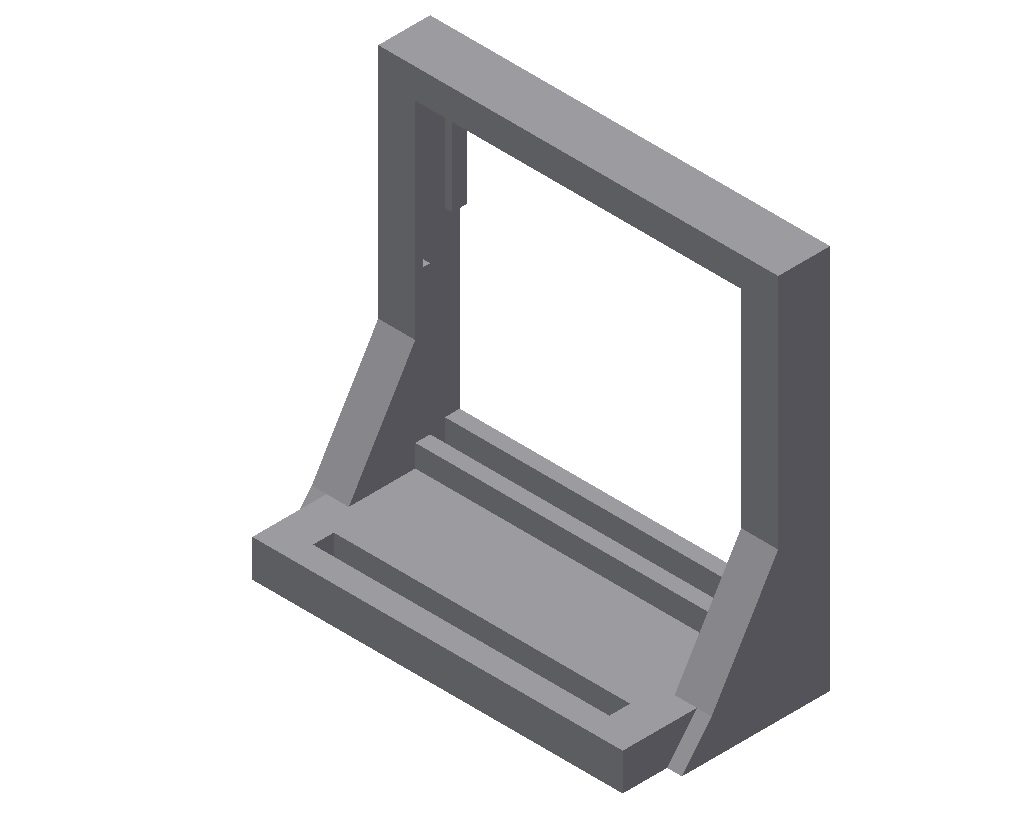
\includegraphics[width=\textwidth]{images/ultrasonicholder-upsidedown.jpg}
	\end{subfigure}
	\caption{The enclosures used to mount the ultrasonic sensors on the chassis}
\end{figure}

The enclosures for the ultrasonic sensors have be designed to place all of the sensors at the same height on each side of the chassis, to ensure that the measurements are similar. The left-most holder is the one which is primarily used.

\begin{figure}[H]
	\centering
	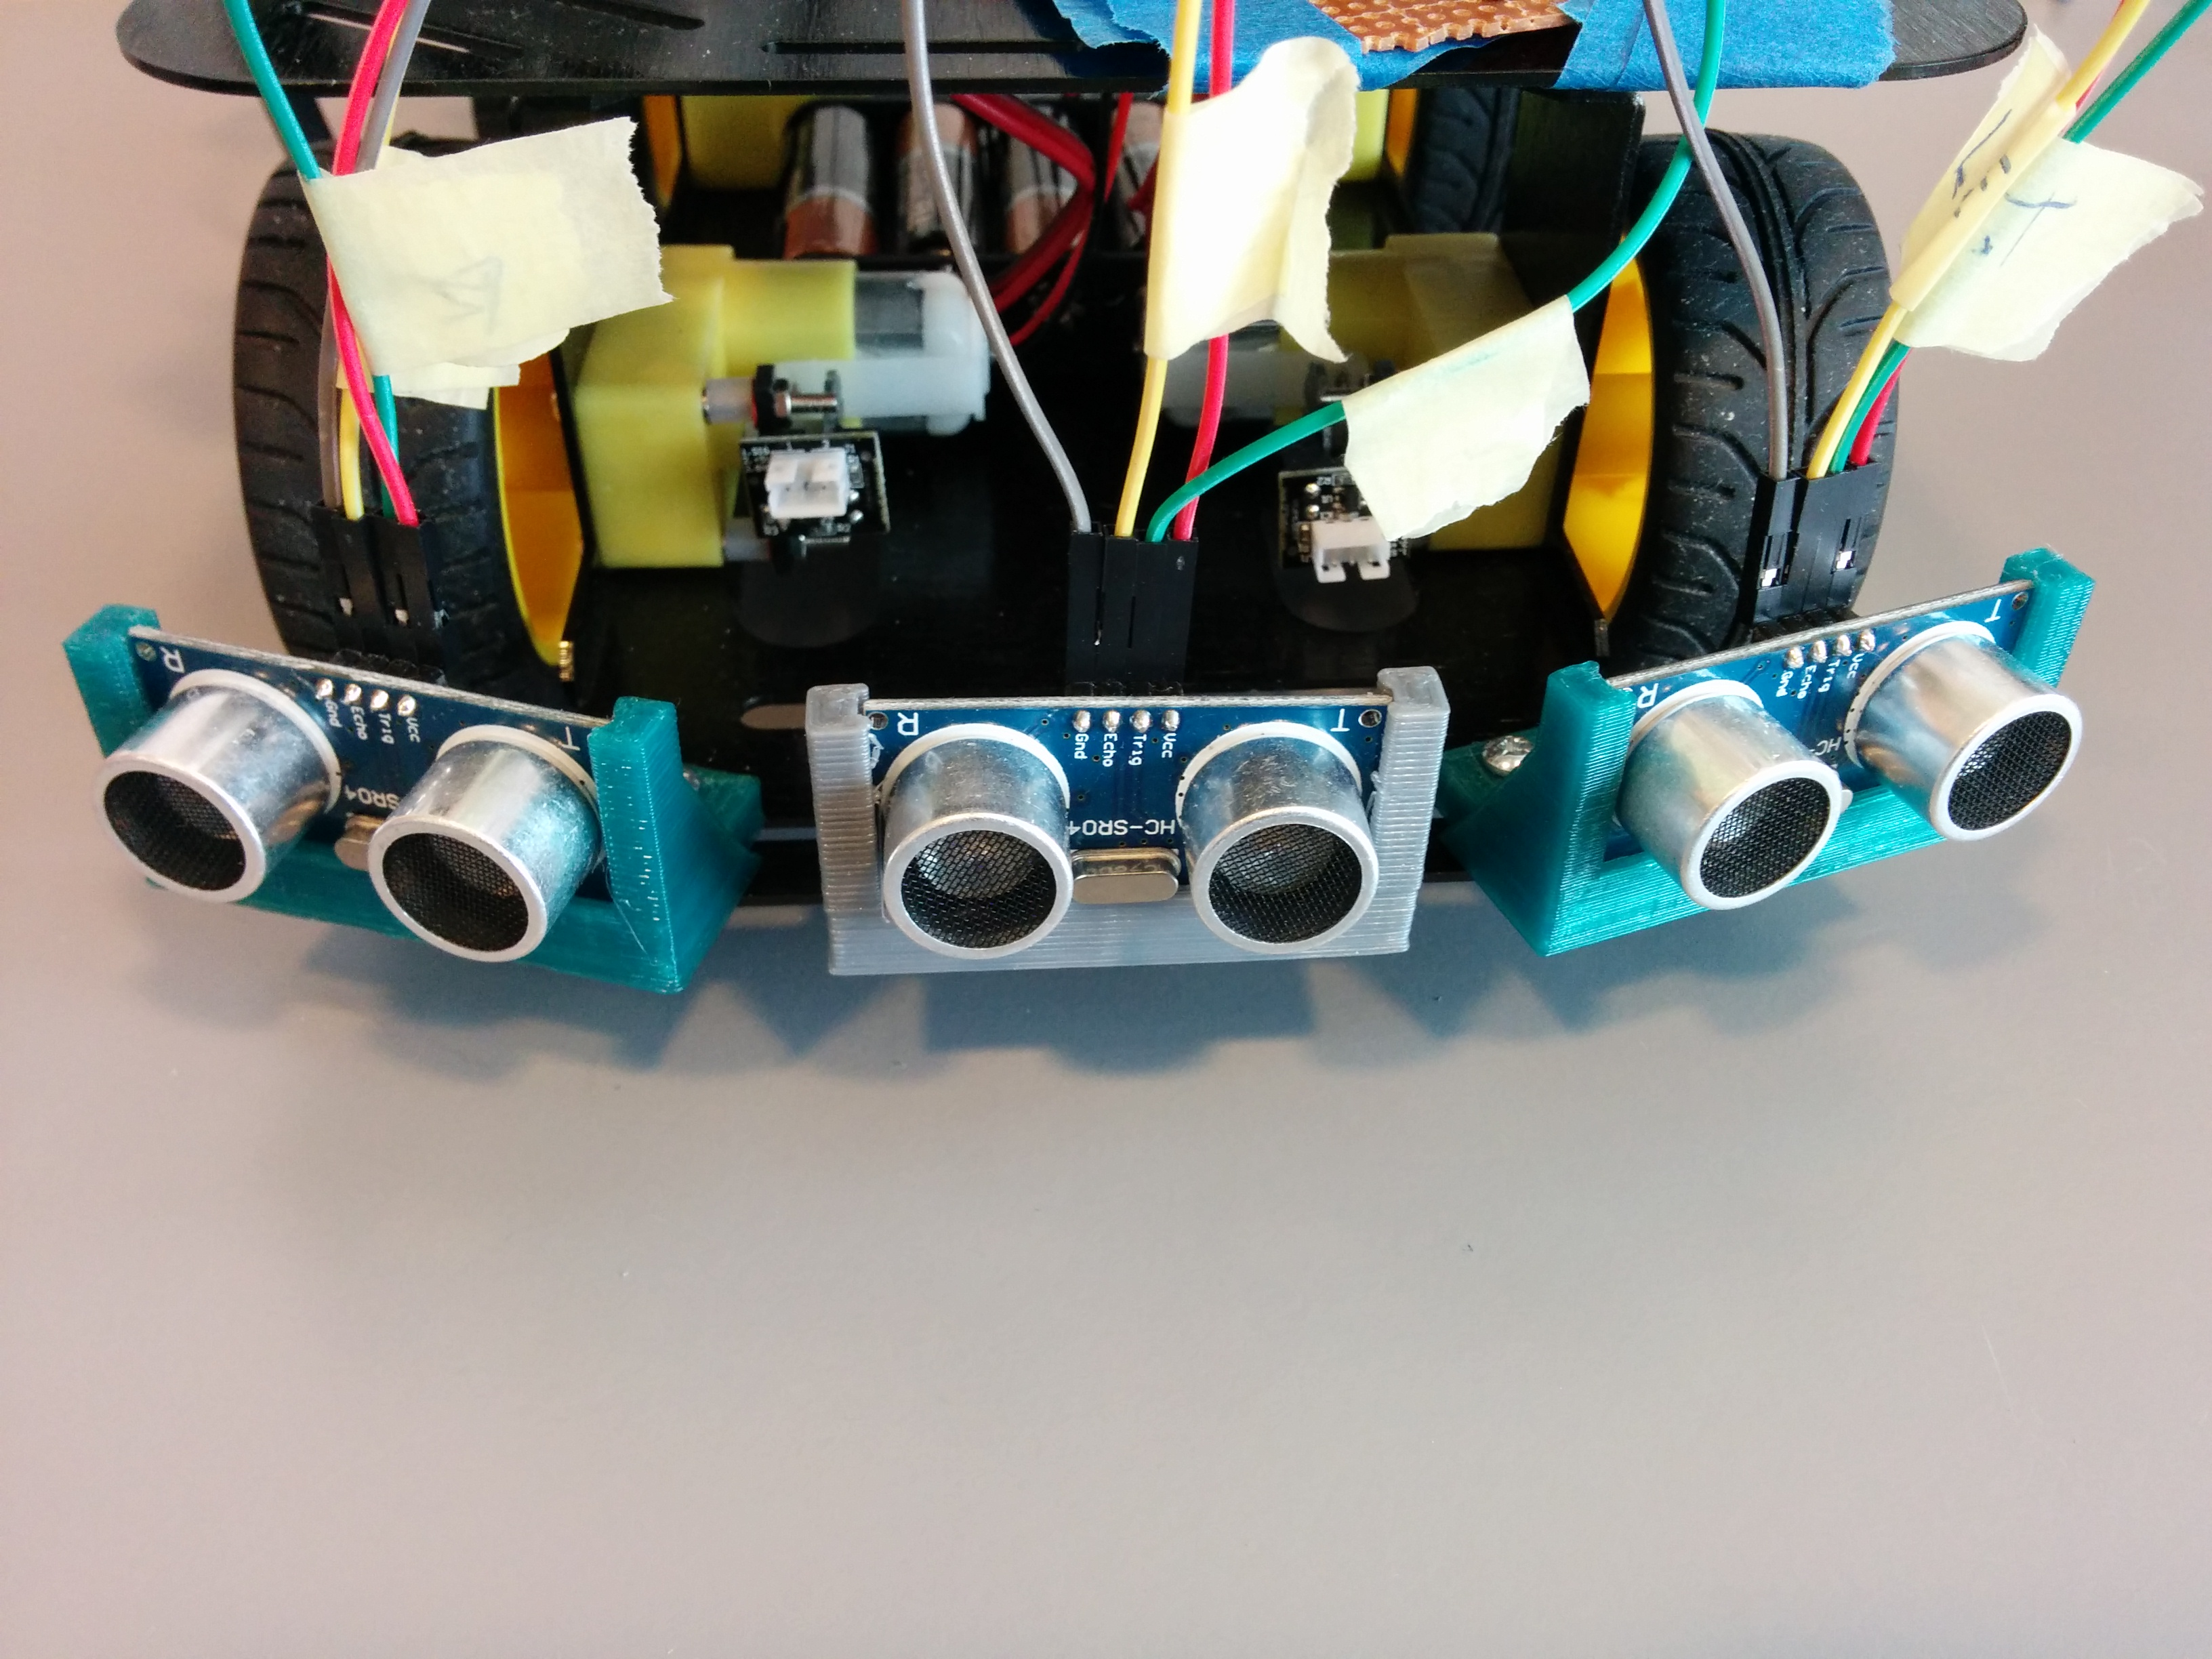
\includegraphics[width=.6\linewidth]{images/mounted_ultrasonic_sensors.jpg}
	\caption{Front view of the mounted ultrasonic sensors}
\end{figure}

The design for the Lidar laser enclosure was found on the internet, modelled by someone who is working on a project using the same Lidar. The enclosure enables the sensor to rotate 360degrees using 3D printed gears that are driven by a stepper motor.\cite{lidarenclosure}.

The enclosure design required a high-end 3D printer due to its size and print time. The prints were completed within a day.

\begin{figure}[H]
	\centering
	\begin{subfigure}[H]{0.4\textwidth}
		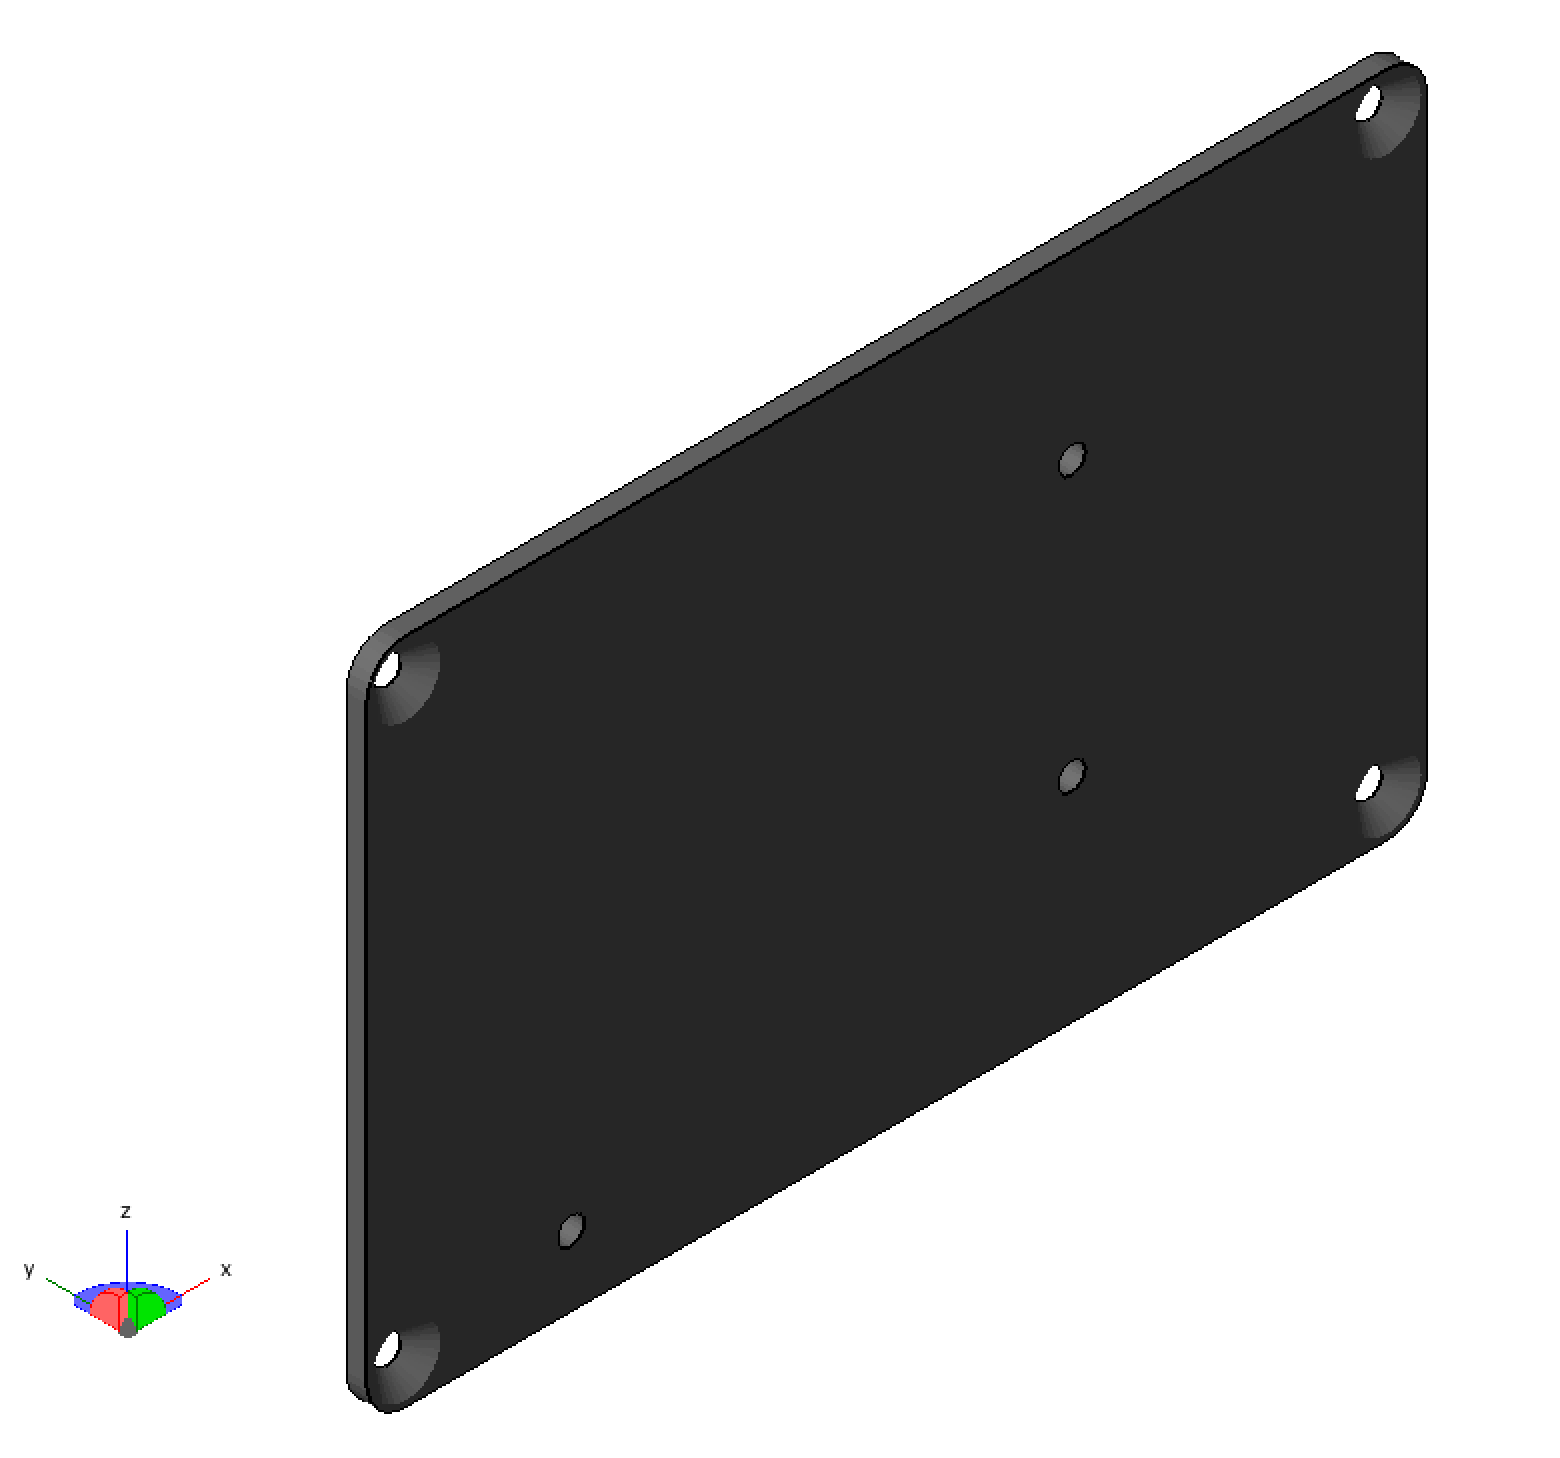
\includegraphics[width=\textwidth]{images/lidarcase-base.png}
	\end{subfigure}%
	\quad
	\begin{subfigure}[H]{0.4\textwidth}
		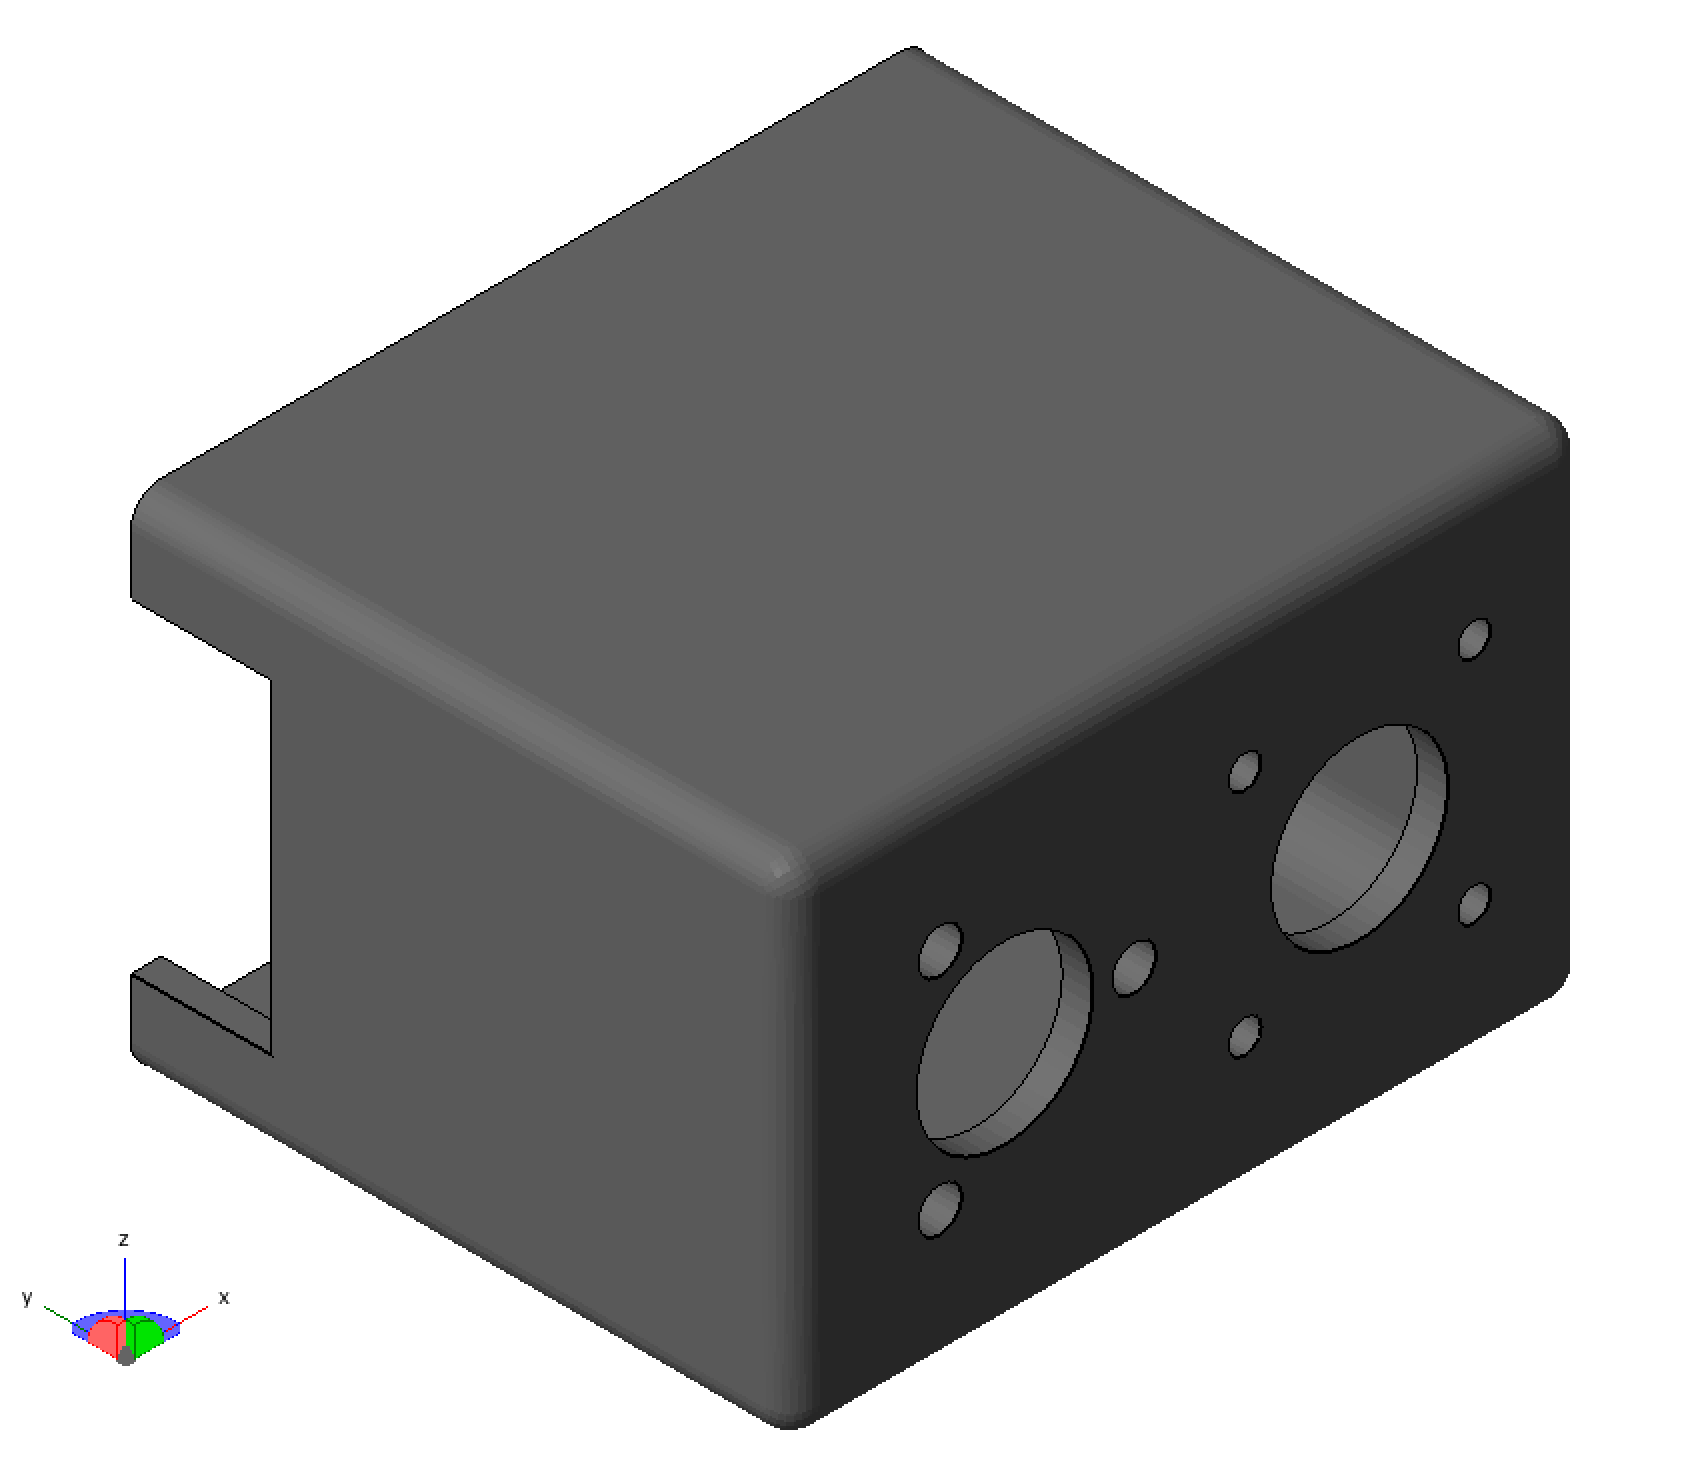
\includegraphics[width=\textwidth]{images/lidarcase-mount.png}
	\end{subfigure}
	\newline
	\begin{subfigure}[H]{0.4\textwidth}
		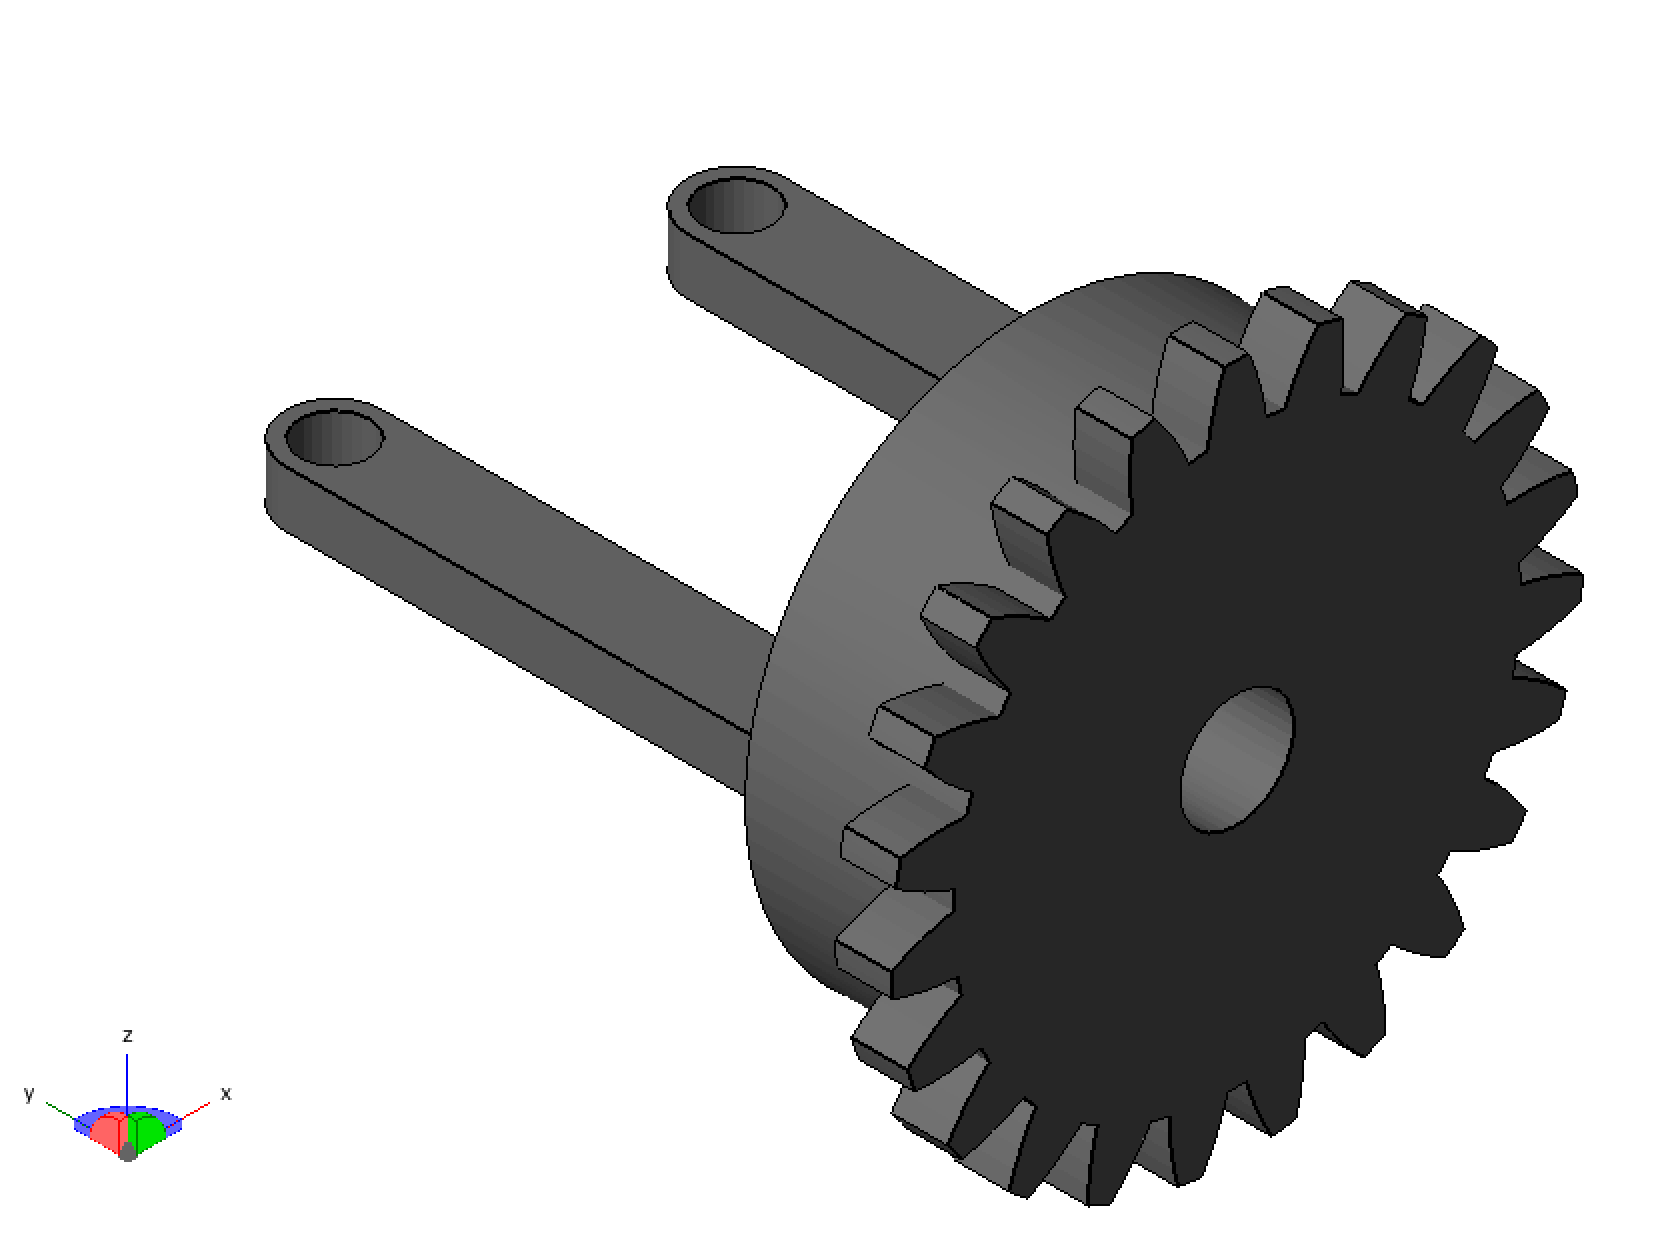
\includegraphics[width=\textwidth]{images/lidarcase-bracket.png}
	\end{subfigure}
	\quad
	\begin{subfigure}[H]{0.4\textwidth}
		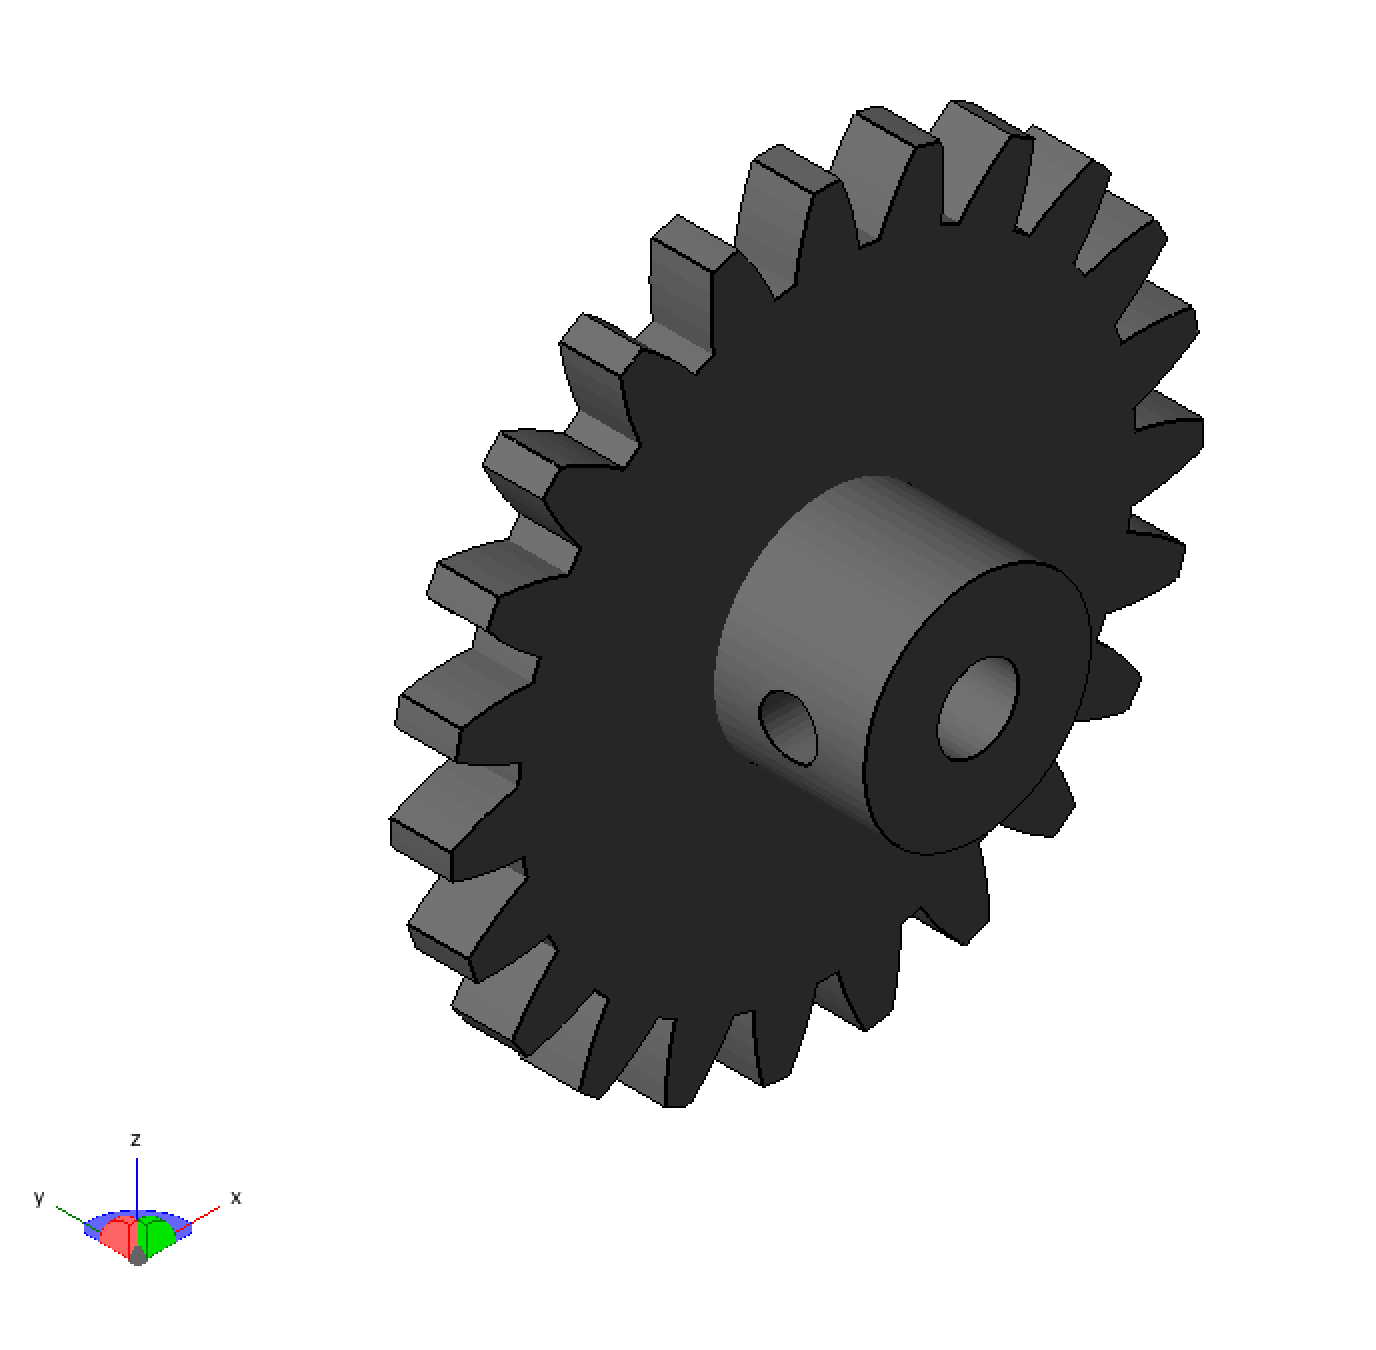
\includegraphics[width=\textwidth]{images/lidarcase-steppergear.png}
	\end{subfigure}
	\caption{Parts of the enclosure used for rotating the LIDAR laser sensor}
\end{figure}

The idea of using a separate enclosure driven by a stepper motor to rotate the laser sensor is to constantly get a 360$\degree$ map of the environment by rotating the sensor separately from the chassis, rather than rotating the chassis to do so. This way, we can also continue to update the map while the rover is on the move. The strength behind using a stepper motor is that it is possible to control each step with great precision, which makes it more reliable when rotating it.

%TODO: Write about assembly
The project ended up being assembled in two separate parts: The rover with the ultrasonic sensors and the Lidar by itself.

\begin{figure}[H]
	\centering
	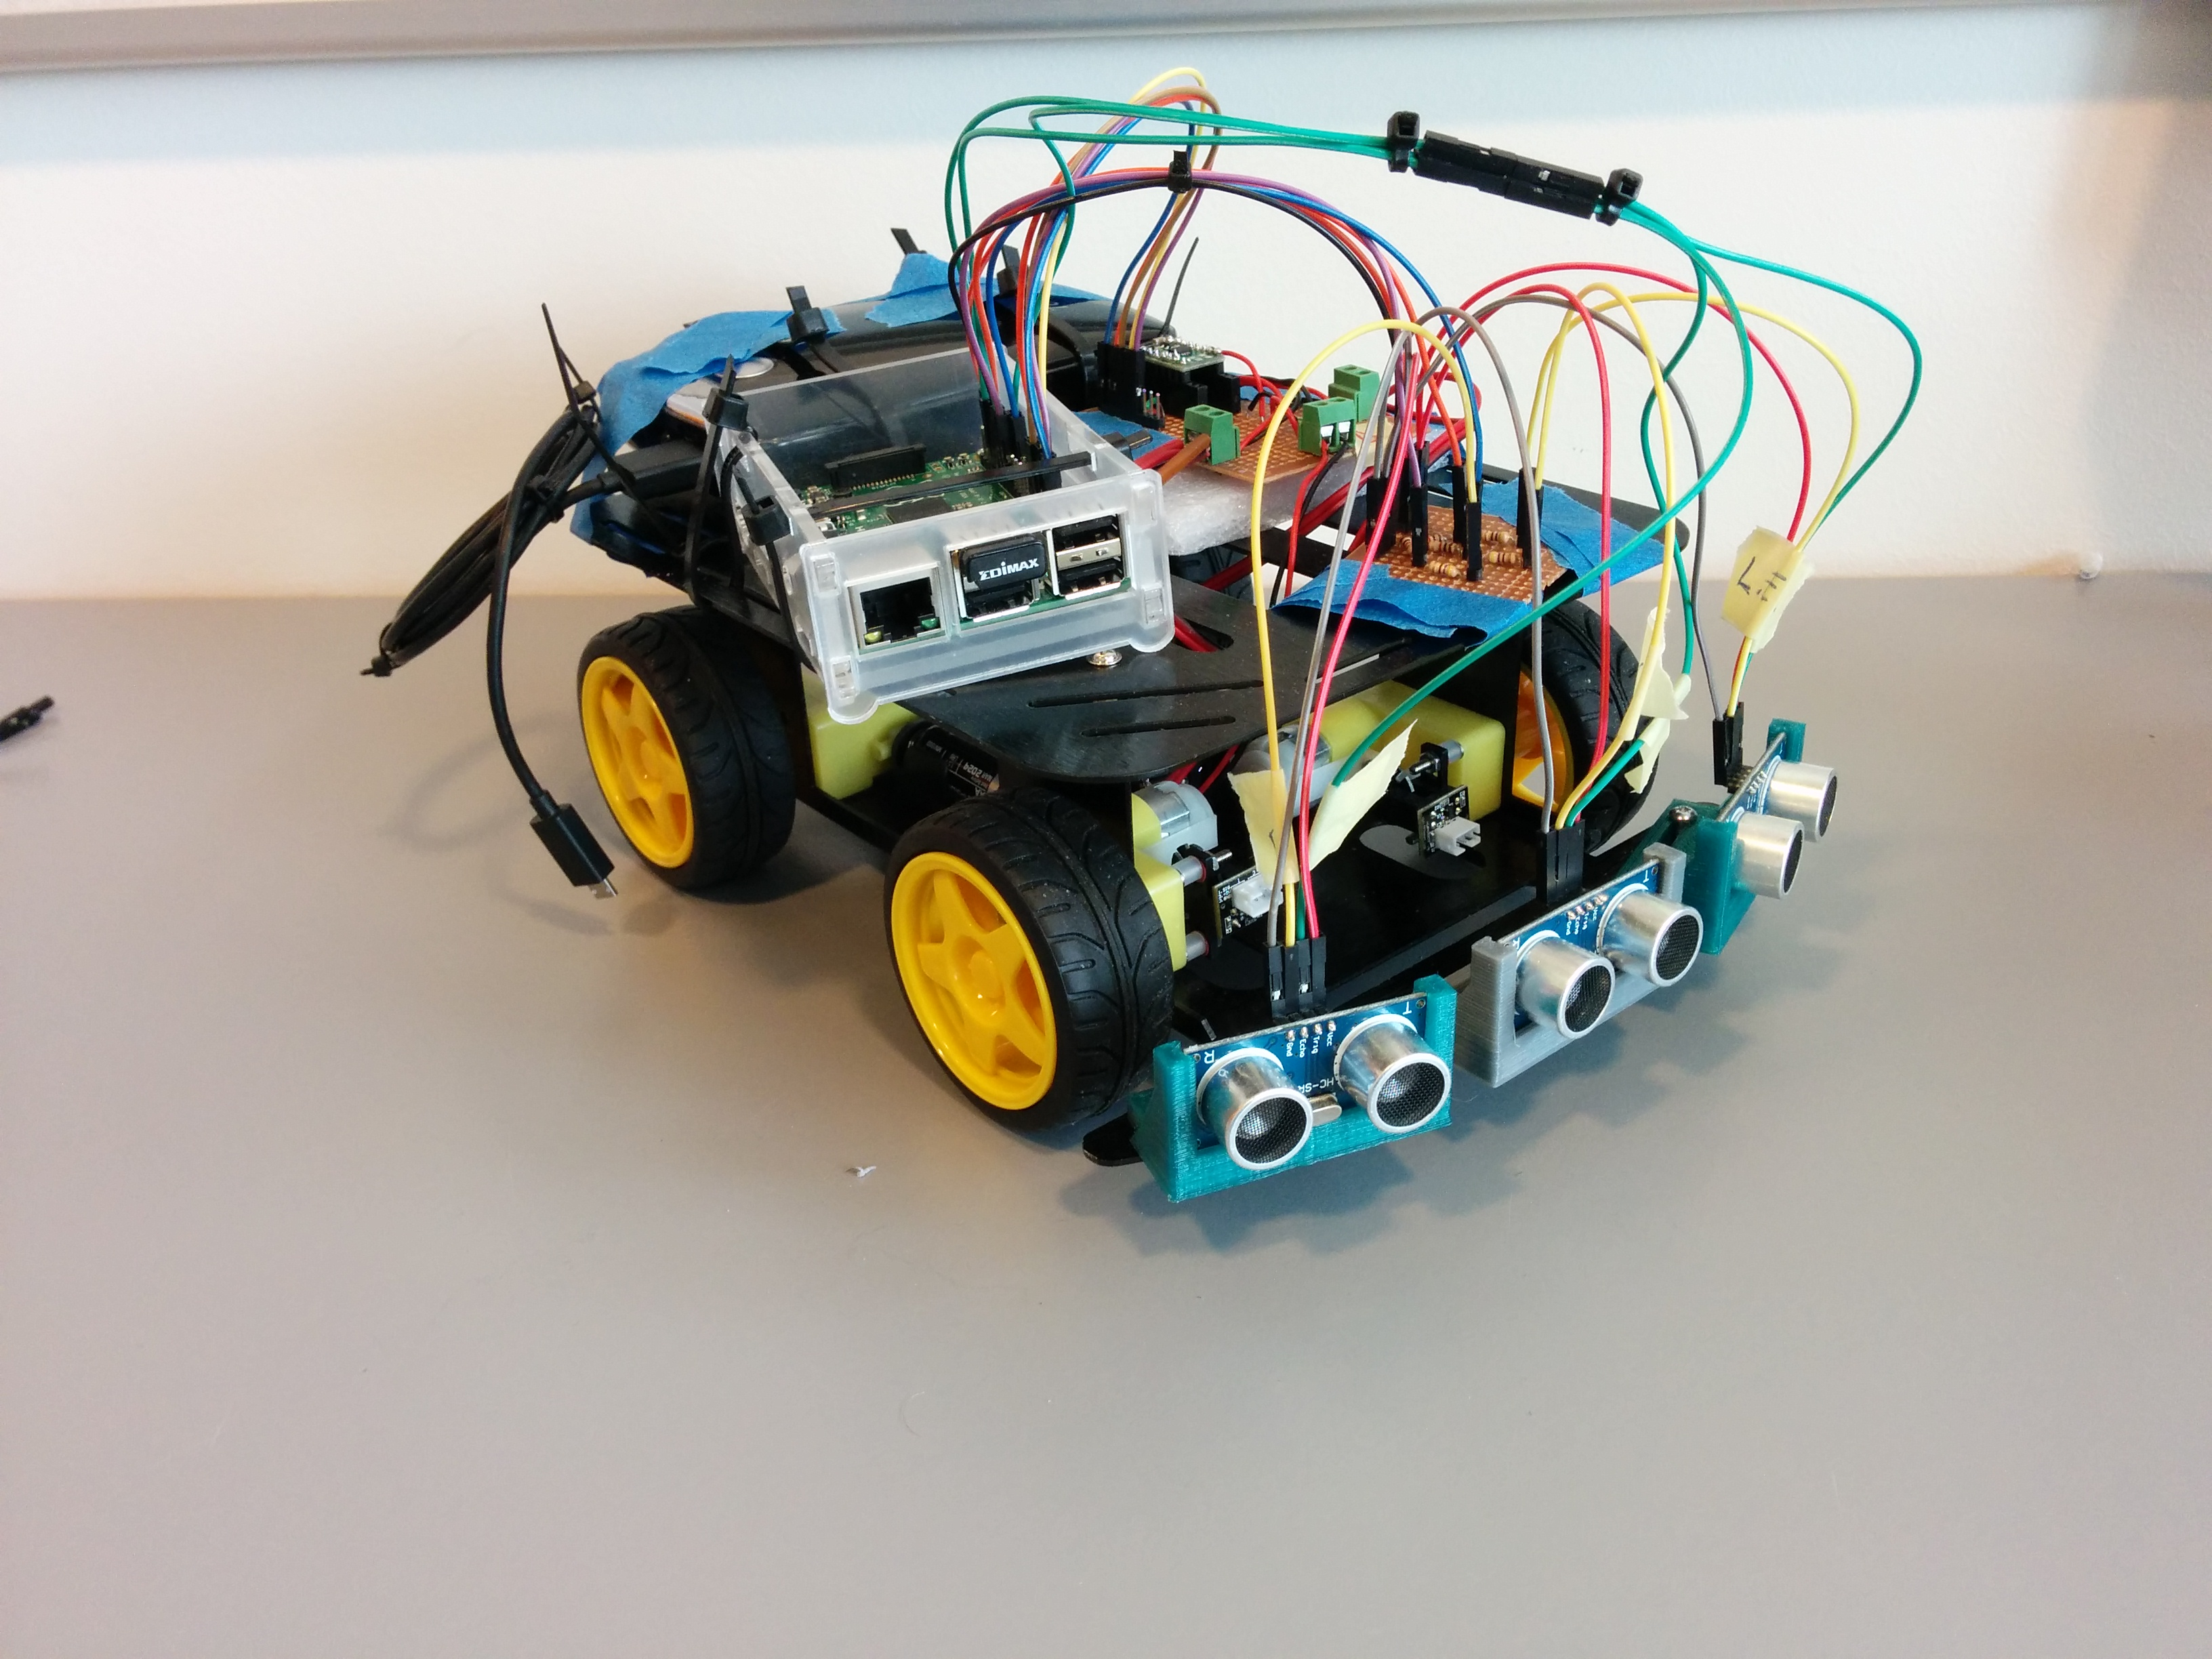
\includegraphics[width=.6\linewidth]{images/build_ultrasonic.jpg}
\end{figure}